% Options for packages loaded elsewhere
\PassOptionsToPackage{unicode}{hyperref}
\PassOptionsToPackage{hyphens}{url}
%
\documentclass[
]{article}
\usepackage{amsmath,amssymb}
\usepackage{lmodern}
\usepackage{ifxetex,ifluatex}
\ifnum 0\ifxetex 1\fi\ifluatex 1\fi=0 % if pdftex
  \usepackage[T1]{fontenc}
  \usepackage[utf8]{inputenc}
  \usepackage{textcomp} % provide euro and other symbols
\else % if luatex or xetex
  \usepackage{unicode-math}
  \defaultfontfeatures{Scale=MatchLowercase}
  \defaultfontfeatures[\rmfamily]{Ligatures=TeX,Scale=1}
\fi
% Use upquote if available, for straight quotes in verbatim environments
\IfFileExists{upquote.sty}{\usepackage{upquote}}{}
\IfFileExists{microtype.sty}{% use microtype if available
  \usepackage[]{microtype}
  \UseMicrotypeSet[protrusion]{basicmath} % disable protrusion for tt fonts
}{}
\makeatletter
\@ifundefined{KOMAClassName}{% if non-KOMA class
  \IfFileExists{parskip.sty}{%
    \usepackage{parskip}
  }{% else
    \setlength{\parindent}{0pt}
    \setlength{\parskip}{6pt plus 2pt minus 1pt}}
}{% if KOMA class
  \KOMAoptions{parskip=half}}
\makeatother
\usepackage{xcolor}
\IfFileExists{xurl.sty}{\usepackage{xurl}}{} % add URL line breaks if available
\IfFileExists{bookmark.sty}{\usepackage{bookmark}}{\usepackage{hyperref}}
\hypersetup{
  pdftitle={Simplified Template for DSI AT2},
  hidelinks,
  pdfcreator={LaTeX via pandoc}}
\urlstyle{same} % disable monospaced font for URLs
\usepackage[margin=1in]{geometry}
\usepackage{graphicx}
\makeatletter
\def\maxwidth{\ifdim\Gin@nat@width>\linewidth\linewidth\else\Gin@nat@width\fi}
\def\maxheight{\ifdim\Gin@nat@height>\textheight\textheight\else\Gin@nat@height\fi}
\makeatother
% Scale images if necessary, so that they will not overflow the page
% margins by default, and it is still possible to overwrite the defaults
% using explicit options in \includegraphics[width, height, ...]{}
\setkeys{Gin}{width=\maxwidth,height=\maxheight,keepaspectratio}
% Set default figure placement to htbp
\makeatletter
\def\fps@figure{htbp}
\makeatother
\setlength{\emergencystretch}{3em} % prevent overfull lines
\providecommand{\tightlist}{%
  \setlength{\itemsep}{0pt}\setlength{\parskip}{0pt}}
\setcounter{secnumdepth}{5}
\ifluatex
  \usepackage{selnolig}  % disable illegal ligatures
\fi

\title{Simplified Template for DSI AT2}
\usepackage{etoolbox}
\makeatletter
\providecommand{\subtitle}[1]{% add subtitle to \maketitle
  \apptocmd{\@title}{\par {\large #1 \par}}{}{}
}
\makeatother
\subtitle{Peter Kiel, modified by Simon Knight And Durand Sinclair}
\author{}
\date{\vspace{-2.5em}22/08/2019}

\begin{document}
\maketitle

{
\setcounter{tocdepth}{2}
\tableofcontents
}
\begin{center}\rule{0.5\linewidth}{0.5pt}\end{center}

\hypertarget{simplified-very-template-for-dsi-at2}{%
\section{Simplified (very) Template for DSI
AT2}\label{simplified-very-template-for-dsi-at2}}

This is the template, or structure for the report. Make sure that you
read it closely, several times.

\textbf{Word length}\\
2800 words (excluding data excerpts and appendices, visualisations, and
references).

\textbf{Citations} In this assignment, use footnotes to do citation.
Here's how to do it. \footnote{This is the text of the footnote which
  you can see at the bottom of the page.}

\textbf{Embedding an image} If you want to embed an image, such as this
UTS logo which is in the same directory as this .Rmd file, here's some
code that shows you how to do it:


\includegraphics{uts_logo_new.png}

\textbf{Structure}\\
This is the suggested structure for your report. The basic structure is
similar to the style of academic papers and, if followed, should ensure
that everything you need to include is present. I have included the
assessment criteria at the relevant places to remind you of what needs
to be in the report.

You are free to vary the structure by renaming the sections, including
other sections, or dropping ones that you don't use. Keep in mind that
the suggested structure is conventional (and therefore easy to follow),
practical, and comprehensive. \emph{(Criterion 5: Professionally
presented in a manner appropriate to the discipline.)}

Note: The text between the angle brackets, \textless{} \textgreater,
below, is replaced by your text.

\begin{center}\rule{0.5\linewidth}{0.5pt}\end{center}

\hypertarget{title-name-student-number-etc}{%
\subsection{Title, name, student number
etc}\label{title-name-student-number-etc}}

\hypertarget{introduction}{%
\subsection{Introduction}\label{introduction}}

\textless a paragraph that gives an overview of what you've
done\textgreater{}

\hypertarget{description-of-process-or-method}{%
\subsection{Description of process, or
method}\label{description-of-process-or-method}}

\textless this is where you give details about what you've been
collecting and how much you data have; why you choose this data to
collect; how you managed the quality and frequency of collection issues;
what you did to anonymise or de-identify the data, and how you dealt
with the storage and sharing of data within the group. Do not include a
dump of all your data here. If you wish to include examples of data (and
I think you should) then put these in an appendix to the report.\\
\emph{Criterion 1: Justifies a method to obtain data from multiple
sources, for gaining insight into a chosen problem, including analysis
of data quality issues in the individual and group data.} \textgreater{}

\hypertarget{analysis}{%
\subsection{Analysis}\label{analysis}}

\textless describe how you analysed your data, and how you contrasted
your data with the group's data.\\
\emph{Criterion 2: Justifies the analysis of the obtained data,
including quality issues, to draw conclusions in a professional and
engaging manner.} You should include your analysis here using R code, or
by loading images and tables you've saved from other programs, like
this.\textgreater{}


\includegraphics{uts_logo_new.png}

Or like this: 
\includegraphics{uts_logo_new.png}

\hypertarget{findings-and-conclusions}{%
\subsection{Findings and conclusions}\label{findings-and-conclusions}}

\textless what conclusions did you come to as a result of the analysis
of your data and of the group's data.\\
\emph{Criterion 2: Justifies the analysis of the obtained data,
including quality issues, to draw conclusions in a professional and
engaging manner.}\textgreater{}

\hypertarget{discussion}{%
\subsection{Discussion}\label{discussion}}

\textless discuss aspects of the process that you see as important. For
example, what difficulties did you encounter; how could you avoid
problems if you did it again; etc\textgreater{}

Your `justification' and evaluation of your approach is likely to go in
this section, but may also be threaded through the preceding sections.
This includes \emph{Criterion 3: Identifies, contextualises, and
reflects on the ethical, privacy, and legal issues relevant to the
collection and analysis of personal data of self and others.}
\textgreater{}

\hypertarget{reflection}{%
\subsection{Reflection}\label{reflection}}

\textless General reflection on what you learnt during this task. What
are you unsure about? What would you do differently if you had to do it
all again? How do these experiences relate to the wider practice of data
science (for example, issues with collecting, cleaning, analysing and
deriving meaning from data, and the ethics of this)? \emph{Criteria 4:
Connects the individual experience of this QS project to the practice of
data science (and the preceding three criteria).}\textgreater{}

\hypertarget{references}{%
\subsection{References}\label{references}}

\textless include any cited references, formatted in Harvard
style.\textgreater{}

\hypertarget{appendices}{%
\subsection{Appendices}\label{appendices}}

\textless include samples of your data - enough to give a sense of what
your raw data looks like\textgreater{}

\hypertarget{other}{%
\subsection{Other}\label{other}}

If you are submitting any additional materials, such as short multimedia
presentations or visualisations (such as Prezi, or voice-over
video/screen capture, etc), they probably can't be submitted through
Canvas so you will need to arrange some other process such as posting on
YouTube or elsewhere, or handing in a memory stick. Please ensure that
additional material like this is accessible to the markers (test this by
accessing it through someone else's computer) and avoid any restrictive
or proprietary software constraints. Remember to check any included web
links!

Diagrams, figures, charts and illustrations must be labelled, and
explained, and must be referred to from somewhere in the report. If
drawn from another source, then the source must be provided.

\hypertarget{the-odi-canvas}{%
\subsection{The ODI Canvas}\label{the-odi-canvas}}

You can download it and include it like this (play around with the
settings to make it display sensibly). You can also include it as a html
file, etc.

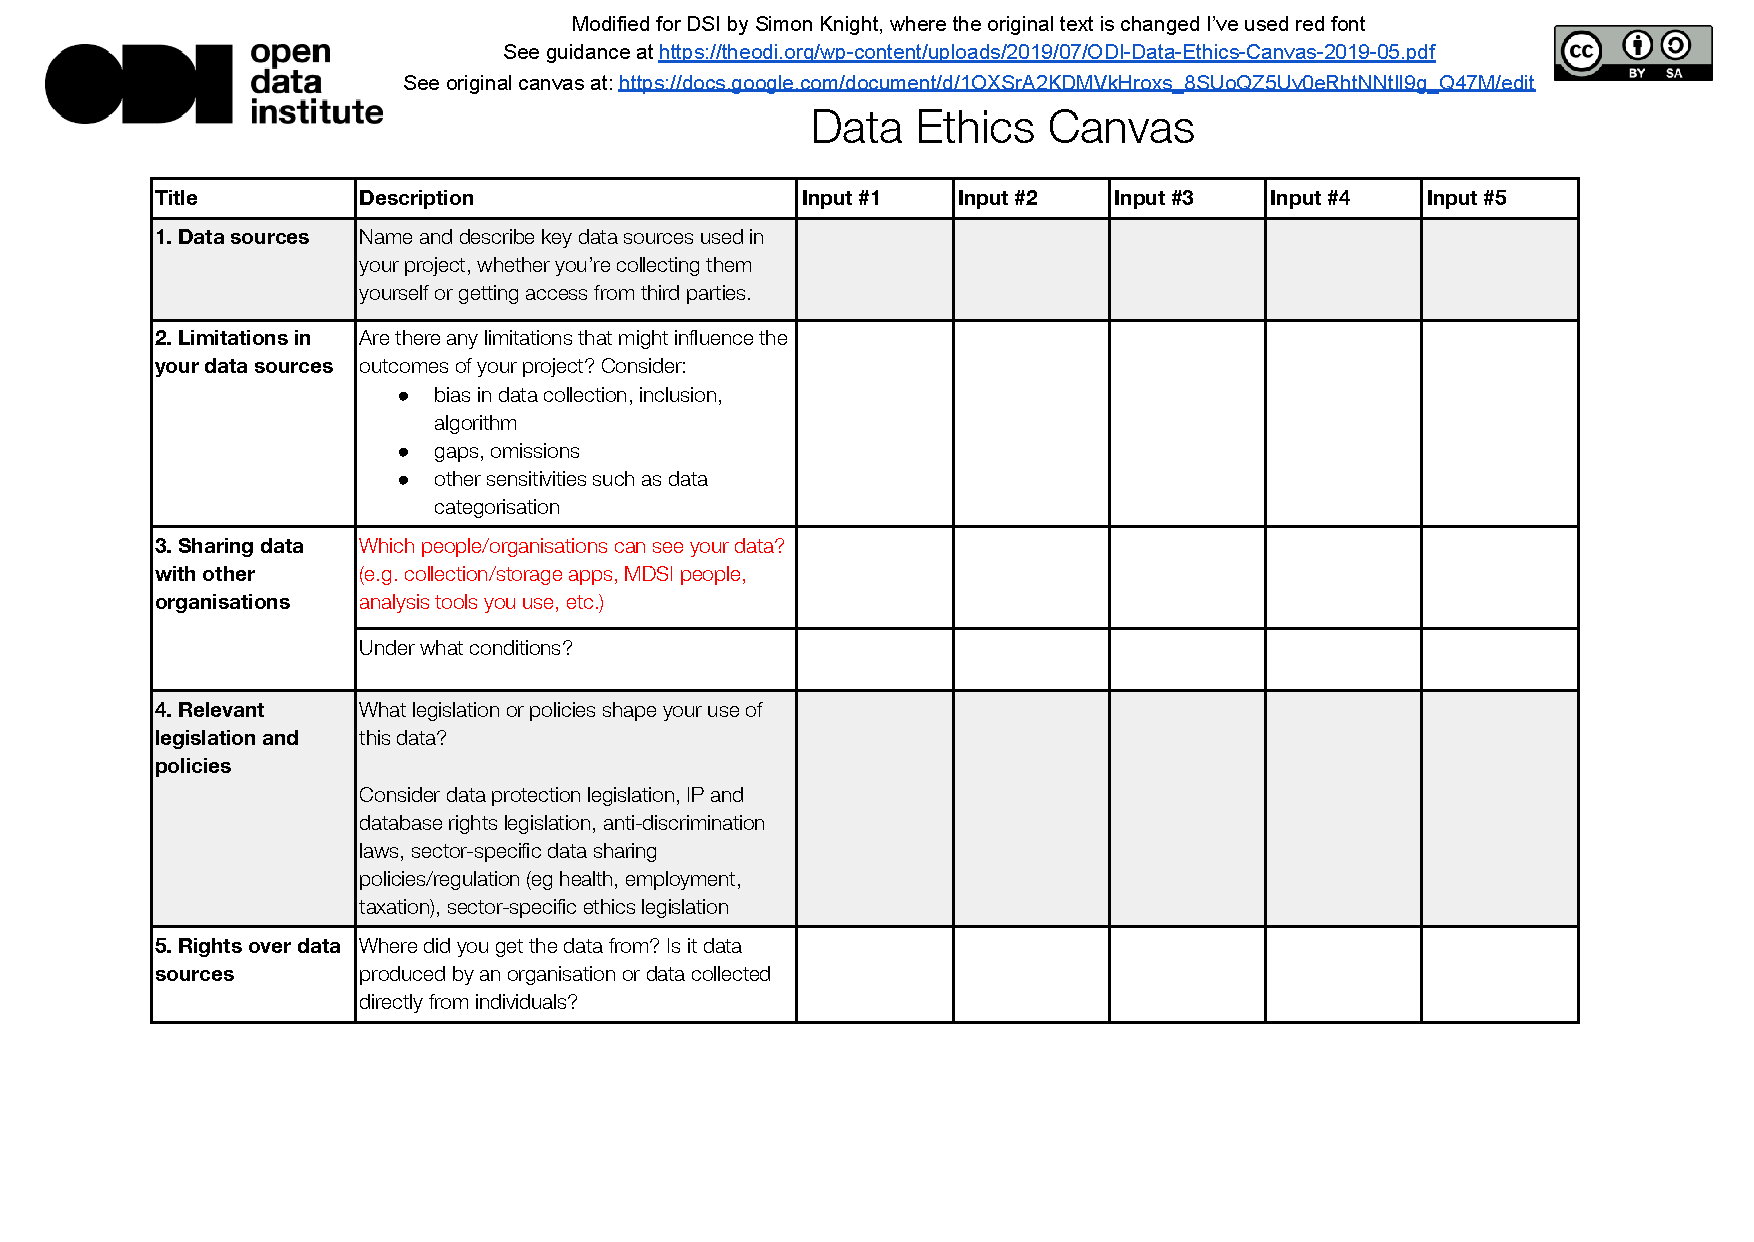
\includegraphics[width=1\linewidth]{DSI_copy_ODI_Data_Ethics_Canvas}

\end{document}
